\section{TWSVM}

TWSVM (孪生支持向量机) 是 Jayadeva 等人于2007年提出的一种改进的双分界面支持向量机,用于解决二分类问题。与传统的支持向量机 (SVM) 不同,TWSVM 为每一类的数据点单独建立一个分类面,其优化策略为,使同一类的数据点尽可能集中的围绕在该类分类面的周围,并且远离另一类数据的分类面。所以 TWSVM 需要解决两个二次规划问题,得到两个不平行的分类面,但是同一类的数据要作为另一个二次规划问题的约束条件,反之亦然。

TWSVM 需要求解以下两个二次优化问题:
\begin{align}
\begin{split}
\label{ts1}
\min_{\mathbf{w}_1,b_1} \; & \frac{1}{2}\|\mathbf{Aw}_1+\mathbf{e}_1b_1\|_2^2+c_1\mathbf{e}_2^T\mathbf{q}_1 \\
s.t.\; & -(\mathbf{Bw}_1+\mathbf{e}_2b_1)+\mathbf{q}_1 \geq \mathbf{e}_2,\mathbf{q}_1\geq 0
\end{split}
\\
\begin{split}
\label{ts2}
\min_{\mathbf{w}_2,b_2} \; & \frac{1}{2}\|\mathbf{Bw}_2+\mathbf{e}_2b_2\|_2^2+c_2\mathbf{e}_1^T\mathbf{q}_2 \\
s.t. \; & (\mathbf{Aw}_2+\mathbf{e}_1b_2)+\mathbf{q}_2\geq \mathbf{e}_1, \mathbf{q}_2\geq 0
\end{split}
\end{align}
其中,$\mathbf{A}_{m_1 \times n}=(\mathbf{a}_1^{(1)},\mathbf{a}_2^{(1)},\ldots,\mathbf{a}_{m_1}^{(1)})^T$ 表示 $m_1$ 个正样本,$\mathbf{B}_{m_2 \times n }=(\mathbf{b}_1^{(2)},\mathbf{a}_2^{(2)},\ldots,\mathbf{a}_{m_2}^{(2)})^T$ 表示 $m_2$ 个负样本,$\mathbf{e}_1$ 和 $\mathbf{e}_2$ 表示相应维数的单位变量,$||\cdot||_2$ 表示L2范数,$\mathbf{q}_1, \, \mathbf{q}_2$ 是松弛向量,$c_1, \, c_2$ 是非负惩罚系数,分别为正样本和负样本的平衡因子,可以用来解决正负样本个数不同的问题。通过求解以上两个优化问题,可以分别得到两个不平行的超平面:
\begin{equation}
\mathbf{x}^T\mathbf{w}_1+b_1=0, \quad \mathbf{x}^T\mathbf{w}_2+b_2=0
\end{equation}
当有一个新的点 $\mathbf{x}$,计算其到两个超平面的垂直距离,如果它距离超平面 $\mathbf{x}^T\mathbf{w}_1+b_1=0$ 的距离小于它到超平面 $\mathbf{x}^T\mathbf{w}_2+b_2=0$ 的距离,则将该点归入正类,否则它属于负类。

我们也可以得到问题 (\ref{ts1})、(\ref{ts2}) 的 Wolfe 对偶问题:
\begin{align}
\begin{split}
\max\limits_{\pmb{\alpha}} \; & \mathbf{e}_2^T \pmb{\alpha}-\frac{1}{2}\pmb{\alpha}^T\mathbf{G}(\mathbf{H}^T\mathbf{H})^{-1}\mathbf{G}^T\pmb{\alpha} \\
s.t. \; & 0 \leq \pmb{\alpha}\leq c_1 \mathbf{e}_2
\end{split}
\\
\begin{split}
\max\limits_{\pmb{\beta}} \; & \mathbf{e}_1^T \pmb{\beta}-\frac{1}{2}\pmb{\beta}^T\mathbf{H}(\mathbf{G}^T\mathbf{G})^{-1}\mathbf{H}^T\pmb{\beta} \\
s.t. \; & 0 \leq \pmb{\beta} \leq c_2\mathbf{e}_1
\end{split}
\end{align}
其中 $\mathbf{\alpha} \in R^{m_2}$ 和 $\mathbf{\beta}\in R^{m_1}$ 是拉格朗日乘子,可以利用 $\mathbf{\alpha}$ 和 $\mathbf{\beta}$ 得到两个不平行的超平面:
\begin{align}
\begin{split}
\mathbf{z}_1 &= (\mathbf{w}^T_1b_1)^T = -(\mathbf{H}^T\mathbf{H})^{-1} \mathbf{G}^
T\pmb{\alpha} \\
\mathbf{z}_2 &= (\mathbf{w}^T_2b_2)^T = (\mathbf{G}^T\mathbf{G})^{-1} \mathbf{H}^T\pmb{\beta}
\end{split}
\end{align}
由于逆矩阵 $(\mathbf{H}^T\mathbf{H})^{-1}$ 和 $(\mathbf{G}^T\mathbf{G})^{-1}$ 可能带来奇异问题,为防止矩阵奇异,可以加入一个正则项 $\varepsilon \mathbf{I}$,$\varepsilon$ 是一个足够小的正数。这样可以保证 $(\mathbf{H}^T\mathbf{H}+\varepsilon \mathbf{I})^{-1}$ 和 $(\mathbf{G}^T\mathbf{G}+\varepsilon \mathbf{I})^{-1}$ 正定,从而不会出现奇异问题。

图 (\ref{twsvm1}) 是对TWSVM的几何解释。
\begin{figure}[ht]
	\centering
	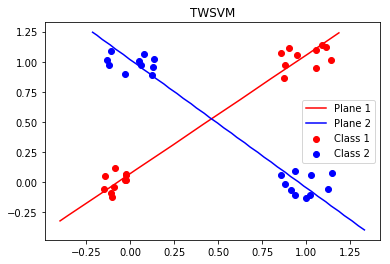
\includegraphics[height=5cm]{./img/TWSVM-img.png}
	\caption{TWSVM}
	\label{twsvm1}
\end{figure}

\section{L1-TWSVM}
TWSVM 有良好的分类性能,已成为数据分类研究的热点。但 TWSVM 使用对离群值较为敏感的 L2 范数来度量距离,导致异常观测点可能会对其结果有较大影响。由于 L1 范数是 L2 范数距离的鲁棒替代 (Ding et al. 2006; Gao 2008; Kwak 2008; Li et al. 2015a; Nie et al. 2015; Wright et al. 2009),本文提出基于 L1 范数的鲁棒分类器。优化问题如下:
\begin{align}
\begin{split}
\label{ts3}
	\min\limits_{\mathbf{w}_1,b_1} \;& \frac{1}{2}||\mathbf{Aw}_1+\mathbf{e}_1b_1||_1+c_1\mathbf{e}_2^T\mathbf{q}_1 \\
	s.t.\;& -(\mathbf{Bw}_1+\mathbf{e}_2b_1)+\mathbf{q}_1 \geq \mathbf{e}_2,\mathbf{q}_1\geq 0
\end{split}
\\
\begin{split}
\label{ts4}
	\min\limits_{\mathbf{w}_2,b_2} \;& \frac{1}{2}||\mathbf{Bw}_2+\mathbf{e}_2b_2||_1+c_2\mathbf{e}_1^T\mathbf{q}_2 \\
	s.t. \; &(\mathbf{Aw}_2+\mathbf{e}_1b_2)+\mathbf{q}_2\geq \mathbf{e}_1, \mathbf{q}_2\geq 0
\end{split}	
\end{align}
其中 $||\cdot||_1$ 表示 L1 范数。在最小化目标函数时,每个平面要尽可能靠近两个分类中的一类,并尽可能远离另一类。由于公式 (\ref{ts3})、(\ref{ts4}) 中不等式为非凸约束,具有局部最优解,可以求解得到两个不平行的超平面:
\begin{align}
	\mathbf{x}^T\mathbf{w}_1+b_1=0, \mathbf{x}^T\mathbf{w}_2+b_2=0
\end{align}
则原问题可优化为:
\begin{align}
\begin{split}
\label{ts5}
	\min\limits_{\mathbf{w}_1,b_1} \;& \frac{1}{2}(\sum_{i=1}^{m_1}\frac{(\mathbf{a}_i^T\mathbf{w}_1+e_1^ib_1)^2}{d_i})+c_1\mathbf{e}_2^T\mathbf{q}_1  \\
	s.t.\;& -(\mathbf{Bw}_1+\mathbf{e}_2b_1)+\mathbf{q}_1 \geq \mathbf{e}_2,\mathbf{q}_1\geq 0
\end{split}
\\
\begin{split}
	\min\limits_{\mathbf{w}_2,b_2} \;& \frac{1}{2}(\sum_{j=1}^{m_2}\frac{(\mathbf{b}_j^T\mathbf{w}_2+e_2^jb_2)^2}{d_j})+c_2\mathbf{e}_1^T\mathbf{q}_2  \\
	s.t. \; &(\mathbf{Aw}_2+\mathbf{e}_1b_2)+\mathbf{q}_2\geq \mathbf{e}_1, \mathbf{q}_2\geq 0
\end{split}
\end{align}
其中 $d_i=|\mathbf{a}_i^T\mathbf{w}_1+e_1^ib_1|\ne 0$,$d_j=|\mathbf{b}_j^T\mathbf{w}_2+e_2^jb_2|\ne 0$,$e_1^i,e_2^j$ 分别表示 $e_1$ 的第 $i$ 个元素和 $e_2$ 的第 $j$ 个元素。由于上述两个式子都包含绝对值运算,难以直接求解,本文提出了一种迭代凸优化策略,基本思想为迭代更新增广向量 $z_1$ 直到连续两次迭代式 (\ref{ts5}) 的目标值小于一个固定值(如0.001),则 $z_1$ 为局部最优解。记 $z_1^p$ 为第 $p$ 次迭代结果,则第 $p+1$ 次迭代结果 $z_1^{(p+1)}$ 可等价为下述问题的解:
\begin{align}
\begin{split}
\label{ts6}
	\min\limits_{\mathbf{z}_1} \;& \frac{1}{2}(\sum_{i=1}^{m_1}\frac{(\mathbf{h}_i^T\mathbf{z}_1)^2}{d_{1i}})+c_1\mathbf{e}_2^T\mathbf{q}_1 \ \\
	s.t.\;& -(\mathbf{Gz}_1+\mathbf{q}_1) \geq \mathbf{e}_2,\mathbf{q}_1\geq 0
\end{split}
\\
\begin{split}
\label{ts7}
	\min\limits_{\mathbf{z}_2} \;& \frac{1}{2}(\sum_{j=1}^{m_2}\frac{(\mathbf{g}_j^T\mathbf{z}_2)^2}{d_{2j}})+c_2\mathbf{e}_1^T\mathbf{q}_2  \\
	s.t. \;& (\mathbf{Hz}_2+\mathbf{q}_2)\geq \mathbf{e}_1, \mathbf{q}_2\geq 0
\end{split}	
\end{align}
其中 $d_{1i}=|\mathbf{h}_i^T\mathbf{z}_1^p|$,$d_{2j}=|\mathbf{g}_j^T\mathbf{z}_2^p|$,$\mathbf{g}_j^T=(\mathbf{b}_j^Te_2^j)$,则公式 (\ref{ts6})、(\ref{ts7}) 可改写为
\begin{align}
\begin{split}
\label{ts8}
	\min\limits_{\mathbf{z}_1} \;& \frac{1}{2}\mathbf{z}_1^T\mathbf{H}^T\mathbf{D}_1\mathbf{Hz}_1+c_1\mathbf{e}_2^T\mathbf{q}_1 \\
	s.t.\;& -(\mathbf{Gz}_1+\mathbf{q}_1) \geq \mathbf{e}_2,\mathbf{q}_1\geq 0
\end{split}
\\
\begin{split}
\label{ts9}
	\min\limits_{\mathbf{z}_2} \;& \frac{1}{2}\mathbf{z}_2^T\mathbf{H}^T\mathbf{D}_2\mathbf{Gz}_2+c_2\mathbf{e}_1^T\mathbf{q}_2 \\
	s.t. \;& (\mathbf{Hz}_2+\mathbf{q}_2)\geq \mathbf{e}_1, \mathbf{q}_2\geq 0
\end{split}
\end{align}
其中 $\mathbf{D}_1=diag(1/d_{11},1/d_{12},…,1/d_{1m_1}),\mathbf{D}_2=diag(1/d_{21},1/d_{22},…,1/d_{2m_2})$ 为对角矩阵。
则问题 (\ref{ts8})、(\ref{ts9}) 等价于:
\begin{align}
\begin{split}
	\min\limits_{\mathbf{z}_1} \;& \frac{1}{2}||\mathbf{Hz}_1||_1+c_1\mathbf{e}_2^T\mathbf{q}_1 \\
	s.t.\;& -(\mathbf{Gz}_1+\mathbf{q}_1) \geq \mathbf{e}_2,\mathbf{q}_1\geq 0
\end{split}
\\
\begin{split}
	\min\limits_{\mathbf{z}_2} \;& \frac{1}{2}||\mathbf{Gz}_2||_1+c_2\mathbf{e}_1^T\mathbf{q}_2 \\
	s.t. \;& (\mathbf{Hz}_2+\mathbf{q}_2)\geq \mathbf{e}_1, \mathbf{q}_2\geq 0
\end{split}
\end{align}
公式 (\ref{ts3}) 是不等式约束(非凸)的凸优化问题,因此它存在解析解。其拉格朗日函数为:
\begin{align}
\begin{split}
	\pmb{L}_1(\mathbf{w}_1,b_1,\mathbf{q}_1,\pmb{\alpha},\pmb{\beta}) &=\frac{1}{2}(\mathbf{Aw}_1+\mathbf{e}_1b_1)^T\mathbf{D}_1(\mathbf{Aw}_1+\mathbf{e}_1b_1)\\
	&+c_1\mathbf{e}_2^T\mathbf{q}_1-\pmb{\alpha}^T(-(\mathbf{Bw}_1+\mathbf{e}_2b_1)+\mathbf{q}_1-\mathbf{e}_2)-\pmb{\beta}^T\mathbf{q}_1
\end{split}
\end{align}
其中 $\pmb{\alpha}=(\alpha_1,\alpha_2,\alpha_3,…,\alpha_{m_2})^T, \pmb{\beta}=(\beta_1,\beta_2,\beta_3,…,\beta_{m_1})^T$ 为拉格朗日乘子,$\pmb{\alpha}\geq 0,\pmb{\beta}\geq 0$,令 $\pmb{L}_1$对$\mathbf{w}_1,b_1,\mathbf{q}_1$ 的偏导分别为0,可得Karush-Kuhn-Tucker (KKT)条件为:
\begin{align}
	&\frac{\partial{L}}{\partial{\mathbf{w}_1}}=\mathbf{A}^T\mathbf{D}_1(\mathbf{Aw}_1+\mathbf{e}_1b_1)+\mathbf{B}^T\pmb{\alpha}=0\\
	&\frac{\partial{L}}{\partial{b_1}}=\mathbf{e}_1^T\mathbf{D}_1(\mathbf{Aw}_1+\mathbf{e}_1b_1)+\mathbf{e}_2\pmb{\alpha}=0\\
	\label{ts10}
	&\frac{\partial{L}}{\partial{\mathbf{q}_1}}=c_1\mathbf{e}_2-\pmb{\alpha}-\pmb{\beta}=0\\
	&-(\mathbf{Bw}_1+\mathbf{e}_2b_1)+\mathbf{q}_1 \geq \mathbf{e}_2, \mathbf{q}_1\geq 0\\
	&\pmb{\alpha}^T(-(\mathbf{Bw}_1+\mathbf{e}_2b_1)+\mathbf{q}_1-\mathbf{e}_2)=0,\pmb{\beta}^T\mathbf{q}_1=0
\end{align}
从式 (\ref{ts10}) 可推出 $0\le \pmb{\alpha} \le c_1\mathbf{e}_2$,结合公式(26)(27)可得:
\begin{align}
	\mathbf{A}^T\mathbf{e}_1^T\mathbf{D}_1(\mathbf{Ae}_1)(\mathbf{w}_1b_1)^T+(\mathbf{B}^T\mathbf{e}_2^T)\pmb{\alpha}=0
\end{align}
结合之前定义的矩阵 $(\mathbf{H,G})$ 及增广向量 $(\mathbf{z}_1,\mathbf{z}_2)$,可以得到
\begin{align}
	\mathbf{H}^T\mathbf{D}_1^p\mathbf{Hz}_1^{(p+1)}+\mathbf{G}^T\pmb{\alpha}=0
\end{align}
即
\begin{align}
\label{ts11}
	\mathbf{z}_1^{(p+1)}=-(\mathbf{H}^T\mathbf{D}_1^p\mathbf{H})^{-1}\mathbf{G}^T\pmb{\alpha}
\end{align}
由于 $(\mathbf{H}^T\mathbf{D}_1^p\mathbf{H})^{-1}$ 为半正定矩阵,因此可能得到不稳定或不准确的解,在实际应用中,本文使用正则化方法(Jayadeva and Chandra (2007), Mangasarian andWild (2006))解决这个问题。$(\mathbf{H}^T\mathbf{D}_1^p\mathbf{H}+\varepsilon \mathbf{I})$ 为正定矩阵 (其中 $\varepsilon$ 为一个小扰动),不受奇点的影响。则逆矩阵 $(\mathbf{H}^T\mathbf{D}_1^p\mathbf{H})^{-1}$ 可由 $(\mathbf{H}^T\mathbf{D}_1^p\mathbf{H}+\varepsilon \mathbf{I})$ 代替,因此 $\mathbf{z}_1^{(p+1)}$ 可推导为:
\begin{align}
	\mathbf{z}_1^{(p+1)}=-(\mathbf{H}^T\mathbf{D}_1^p\mathbf{H}+\varepsilon \mathbf{I})^{-1}\mathbf{G}^T\pmb{\alpha}
\end{align}
同样的
\begin{align}
	\mathbf{z}_2^{(p+1)}=-(\mathbf{G}^T\mathbf{D}_2^p\mathbf{G}+\varepsilon \mathbf{I})^{-1}\mathbf{H}^T\pmb{\beta}
\end{align}
将增广向量 $\mathbf{z}_1^{(p+1)},\mathbf{z}_2^{(p+1)}$ 分别代入拉格朗日函数中。在KKT条件下,原问题 (\ref{ts3})、(\ref{ts4}) 转变为 Wolfe 对偶问题:
\begin{align}
\begin{split}
	\max \limits_{\pmb{\alpha}} \;& \mathbf{e}_2^T\pmb{\alpha}-\frac{1}{2}\pmb{\alpha}^T\mathbf{G}(\mathbf{H}^T\mathbf{D}_1\mathbf{H})^{-1}\mathbf{G}^T\pmb{\alpha} \\
	s.t.\;& 0\le \pmb{\alpha} \le c_1\mathbf{e}_2
\end{split}
\\
\begin{split}		
	\max \limits_{\pmb{\beta}} \;& \mathbf{e}_1^T\pmb{\beta}-\frac{1}{2}\pmb{\beta}^T\mathbf{H}(\mathbf{G}^T\mathbf{D}_2\mathbf{G})^{-1}\mathbf{H}^T\pmb{\beta} \\
	s.t.\;& 0\le \pmb{\beta} \le c_2\mathbf{e}_1
\end{split}
\end{align}
通过求解对偶问题可得拉格朗日乘子 $\pmb{\alpha} \in \pmb{R}^{m_2\times 1},\pmb{\beta} \in \pmb{R}^{m_1\times 1}$ 以及权向量 $\mathbf{w}_1,\mathbf{w}_2$、偏差 $b_1,b_2$,即获得两个不平行的超平面。
对于新加入的点 $\mathbf{x}\in \mathbf{R}^n$,根据决策方程 $f(\mathbf{x})$ (选择最近的超平面) 将其分配到对应类别中
\begin{align}
	f(\mathbf{x})=arg \min\limits_{i=1,2} \;(|\mathbf{x}^T\mathbf{w}_i+b_i|/|||\mathbf{w}_i|)
\end{align}
其中 $|\cdot|$ 表示取绝对值。
式 (\ref{ts3}) 中的目标函数为非凸约束的凸问题,因此 $\mathbf{z}_1^{(p+1)}$ 为此问题的局部最优解。而在式 (\ref{ts11}) 中,$\mathbf{D}_1^p$ 依赖于 $\mathbf{z}_1^{(p+1)}$,因此它是一个未知变量,可看作 (\ref{ts3}) 中目标的隐变量,可以同相同的迭代算法交替优化求解。我们根据前一次迭代结果 $\mathbf{z}_1^{(p+1)}$ 来更新 $\mathbf{D}_1^p$,又通过 $\mathbf{D}_1^p$ 来改变 $\mathbf{z}_1^{(p+1)}$,增加p直到连续两次迭代结果小于一个固定值。此外,适当的初始化可有效加快算法收敛速度。本文通过求解公式 (\ref{ts1})、(\ref{ts2})得到初始解,仿真结果较优。算法1总结了L1-TWSVM的迭代过程。